\documentclass[notitlepage]{article}
%twocolumn for two columns saves space

\usepackage{amsmath}
\usepackage{fullpage}
\usepackage{graphicx}
\usepackage{hyperref}
\usepackage{subcaption}
\usepackage{amsfonts}
\usepackage{booktabs}

% https://tex.stackexchange.com/questions/8625/force-figure-placement-in-text
\usepackage{parskip}

% space saving
\usepackage[text={16cm,24cm}]{geometry}
\usepackage[compact]{titlesec}
\usepackage{mathptmx}

\usepackage[backend=biber,style=ieee,sorting=ynt]{biblatex}
\bibliography{citation}

% https://tex.stackexchange.com/questions/111948/what-is-a-overfull-hbox-9-89561pt-too-wide
\sloppy

\title{IYSE6420: BirdCLEF Birdcall Distribution Maps}

%% Authors
\author{
    Anthony Miyaguchi \texttt{<acmiyaguchi@gatech.edu>}
}

\begin{document}
\maketitle
\thispagestyle{empty}

\begin{abstract}

We utilize geospatial features of bird call metadata from the BirdCLEF 2022 competition to derive a distribution map for a subset of species in California and the Western United States.
We build several Bayesian models that incorporates species frequency information and remote sensing data from USGS and NASA in a regular lattice built from area-of-interest (AOI) geometries, using both hierarchical modeling to incorporate information across a subset of species and a conditional autoregressive (CAR) distribution for spatial random effects.
We generate several species distribution maps and make qualitative comparisons against known distribution maps.
All code and data is available on-request, and may be available publicly on Github/GCP pending permission from course instructors.

\end{abstract}

\section{Introduction}

We are interested in whether we can produce and analyze species distribution map using Bayesian methods.

The BirdCLEF Challenge is a year competition held as part of the Conference and Labs of the Evaluation Forum.
The purpose of the challenge is to classify bird call segments and species from soundscapes captured from audio recording devices deployed in the fields.
The competition hosts provide a training dataset derived from xeno-canto, a crowd-sourced platform for sharing user-generated recordings of bird calls from around the world.

\section{Dataset}
\subsection{BirdCLEF 2022 Training Metadata}

The BirdCLEF 2022 competition provides over 14,800 recordings from 152 species \cite{kahl2022overview}.
We are interested in the spatial features from the recording metadata, which are the latitude and longitude of the recording.
The recordings in the competition dataset are drawn from the xeno-canto library, but it does not reflect the entirety of the library.
Each species is capped to 500 recordings in the dataset, with frequency of recordings generally correlated with their rarity in nature and population density among other factors.

\subsection{Google Earth Engine}

Google Earth Engine is a cloud-based platform for processing geospatial data \cite{gorelick_google_2017}.
We use remote sensing data from the United States Geological Survey (USGS) and the National Aeronautics and Space Administration (NASA) to obtain elevation, temperature, land cover classification, and population density data from various sources hosted on Earth Engine.

Elevation data is derived from the NASA Shuttle Radar Topography Mission dataset (\texttt{USGS/SRTMGL1\_003}) \cite{nasa_srtmg}.
Temperature data is derived from the MODIS/Terra Land Surface Temperature/Emissivity dataset (\texttt{MODIS/006/MOD11A1}) \cite{wan_zhengming_mod11a1_2015}.
Land cover classification data is derived from the MODIS/Terra+Aqua Land Cover Type dataset (\texttt{MODIS/006/MCD12Q1}) \cite{friedl_mark_mcd12q1_2019}.
Population density data is derived from the Gridded Population of the World, Version 4 dataset (\texttt{CIESIN/GPWv411/GPW\_Population\_Density}) \cite{gpwv4}.

We generate a regular lattice of polygons from area-of-interest (AOI) geometries which are used to derive a dataset for a region at a fraction of a degree resolution.
We choose California and the Western United States as our AOI, due to familiarity with the region and diversity of geography and climate.
The dataset is generated over each polygon in the lattice and computing an aggregate statistic from each data source.

\section{Methodology}

\subsection{Conditional Autoregressive Distribution}

The likelihood for a conditional autoregression (CAR) distribution is given by the following equation:

\begin{equation}
f(x|W, \alpha, \tau) =
    \frac{|T|^{1/2}}{(2\pi)^{k/2}}
    \exp \left\{
        -\frac{1}{2} (x - \mu)^\prime T^{-1} (x - \mu)
    \right\}
\end{equation}

where

\begin{equation}
\begin{aligned}
    T &= (\tau D (I-\alpha W))^{-1} \\
    D &= diag(\sum_{i} W_{ij})
\end{aligned}
\end{equation}


This is a special form of the multivariate normal with with a covariance matrix that captures the adjacency structure of the neighborhood graph. 
PyMC provides this distribution out-of-the-box, which we utilize for spatial random effects \cite{salvatier_probabilistic_2016}.


\subsection{Hierarchical Modeling}

We try out a variety of Poisson Generalized Linear Models (GLMs) for developing our distribution map.
There are three main components to these models: an intercept term, a feature term, and a random spatial effects term.
We take advantage of heirachical and multi-level modeling techniques to both pool (or share) and vary information across observations, species, and geographical grid indices.

TODO: write out three models

\begin{figure}[hbt!]
\centering
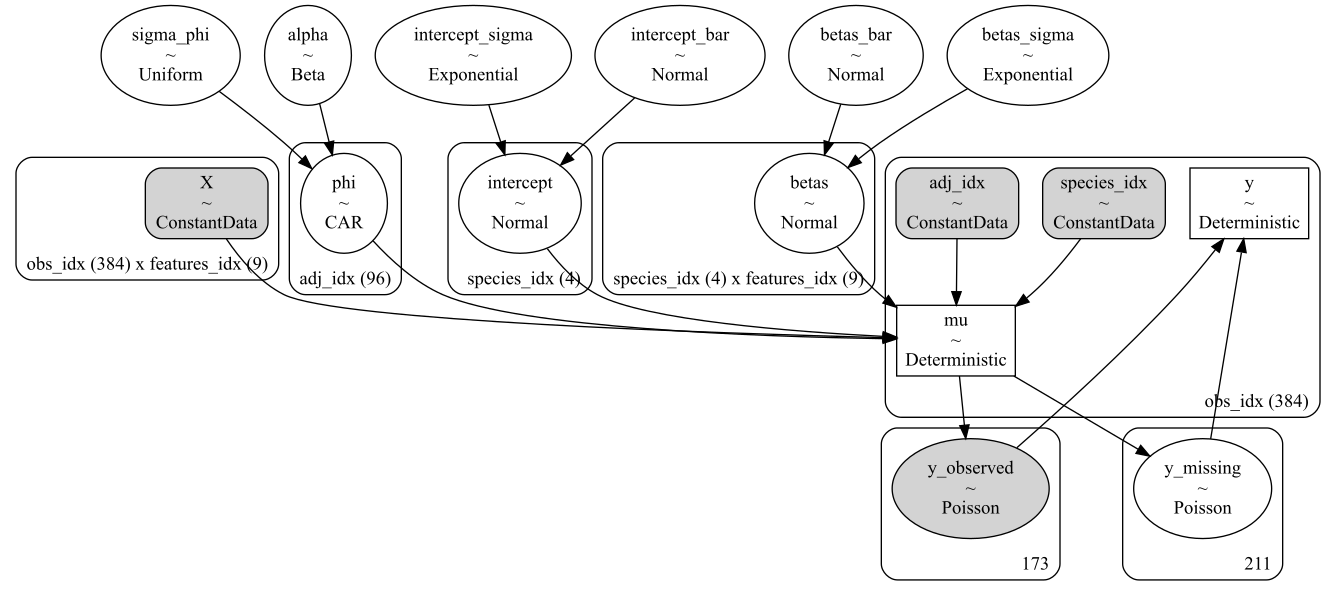
\includegraphics[width=\textwidth]{report/figures/full_model.png}
\caption{Varying intercept, varying covariate, CAR model}
\end{figure}

We compare the models using the widely applicable information criterion (WAIC) on a deviance scale to choose our final model.
These models are discussed in more detail during model selection \ref{model_selection}.

\section{Data and Analysis}

\subsection{Stochastic Search Variable Selection}

There are a total of 27 features that are available for modeling.
Many of these features, such as land cover classification, may have a significant degree of skewness affecting the fitted model.
We use a stochastic search variable selection (SSVS) to inform our choice of feature transformation.
In our first model, we lkj

\begin{figure}[hbt!]
\centering
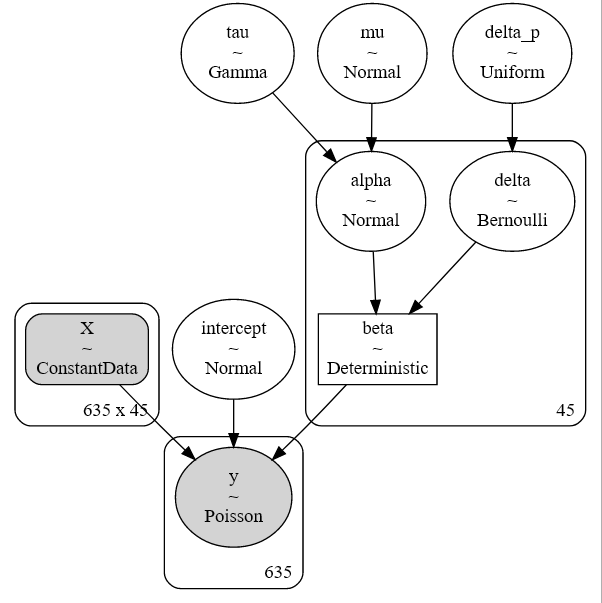
\includegraphics[width=0.5\textwidth]{report/figures/svss_model.png}
\end{figure}

\begin{figure}[hbt!]
\centering
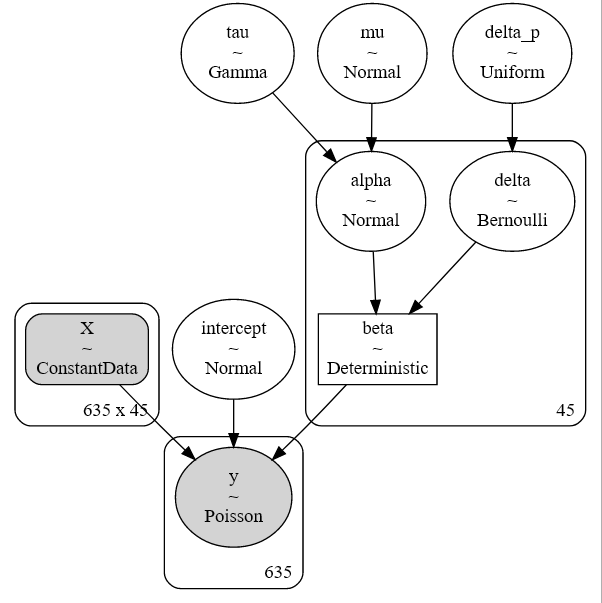
\includegraphics[width=\textwidth]{report/figures/svss_model.png}
\end{figure}


\begin{figure}[hbt!]
\centering
\begin{tabular}{llr}
\toprule
{} &                                        feature &  probability \\
\midrule
0 &  000010110000000000010010000100011001111100000 &     0.000450 \\
1 &  100010110000000000000000000100010101111100001 &     0.000425 \\
2 &  100010110000000000000000000100011101111100001 &     0.000350 \\
3 &  000010110000000000000010000100011101111100001 &     0.000325 \\
4 &  000011010000000000000000000110011001111100000 &     0.000250 \\
\bottomrule
\end{tabular}
\caption{Top models with Poisson GLM with unscaled and log-scaled covariates.}
\end{figure}


\begin{figure}[hbt!]
\centering
\begin{tabular}{lrrrrl}
\toprule
{} &   mean &     sd &  hdi\_3\% &  hdi\_97\% &        feature\_name \\
\midrule
delta[0]  &  0.993 &  0.084 &     1.0 &      1.0 &  population\_density \\
delta[1]  &  0.674 &  0.469 &     0.0 &      1.0 &        elevation\_p5 \\
delta[2]  &  0.601 &  0.490 &     0.0 &      1.0 &       elevation\_p50 \\
delta[3]  &  0.619 &  0.486 &     0.0 &      1.0 &       elevation\_p95 \\
delta[4]  &  1.000 &  0.000 &     1.0 &      1.0 &      LST\_Day\_1km\_p5 \\
delta[5]  &  0.857 &  0.350 &     0.0 &      1.0 &     LST\_Day\_1km\_p50 \\
delta[6]  &  0.733 &  0.442 &     0.0 &      1.0 &     LST\_Day\_1km\_p95 \\
delta[7]  &  1.000 &  0.000 &     1.0 &      1.0 &    LST\_Night\_1km\_p5 \\
delta[8]  &  0.651 &  0.477 &     0.0 &      1.0 &   LST\_Night\_1km\_p50 \\
delta[9]  &  0.588 &  0.492 &     0.0 &      1.0 &   LST\_Night\_1km\_p95 \\
delta[10] &  0.991 &  0.094 &     1.0 &      1.0 &       land\_cover\_01 \\
delta[11] &  0.478 &  0.500 &     0.0 &      1.0 &       land\_cover\_02 \\
delta[12] &  0.778 &  0.416 &     0.0 &      1.0 &       land\_cover\_03 \\
delta[13] &  0.975 &  0.158 &     1.0 &      1.0 &       land\_cover\_04 \\
delta[14] &  0.983 &  0.130 &     1.0 &      1.0 &       land\_cover\_05 \\
delta[15] &  0.932 &  0.253 &     0.0 &      1.0 &       land\_cover\_06 \\
delta[16] &  0.879 &  0.326 &     0.0 &      1.0 &       land\_cover\_07 \\
delta[17] &  1.000 &  0.000 &     1.0 &      1.0 &       land\_cover\_08 \\
delta[18] &  0.991 &  0.095 &     1.0 &      1.0 &       land\_cover\_09 \\
delta[19] &  0.892 &  0.311 &     0.0 &      1.0 &       land\_cover\_10 \\
delta[20] &  1.000 &  0.007 &     1.0 &      1.0 &       land\_cover\_11 \\
delta[21] &  1.000 &  0.000 &     1.0 &      1.0 &       land\_cover\_12 \\
delta[22] &  0.708 &  0.455 &     0.0 &      1.0 &       land\_cover\_13 \\
delta[23] &  0.388 &  0.487 &     0.0 &      1.0 &       land\_cover\_14 \\
delta[24] &  0.480 &  0.500 &     0.0 &      1.0 &       land\_cover\_15 \\
delta[25] &  0.422 &  0.494 &     0.0 &      1.0 &       land\_cover\_16 \\
delta[26] &  0.972 &  0.165 &     1.0 &      1.0 &       land\_cover\_17 \\
\bottomrule
\end{tabular}
\caption{Probability that a feature is included in a model via SSVS. We note that population density and land cover classification features are log-scaled.}
\end{figure}

\begin{figure}[hbt!]
\centering
\begin{tabular}{llr}
\toprule
{} &                      feature &  probability \\
\midrule
0 &  111111111111111111111111111 &     0.050600 \\
1 &  111111111111111111111110111 &     0.013237 \\
2 &  111111111111111111111111011 &     0.012725 \\
3 &  111111111111111111111111101 &     0.009838 \\
4 &  111111111110111111111111111 &     0.008563 \\
\bottomrule
\end{tabular}
\caption{Top models with Poisson GLM with unscaled elevation and temperature covariates, and log-scaled population density and land cover classification covariates.}
\end{figure}

\subsection{Model Selection}
\label{model_selection}

\begin{figure}[ht!]
\centering
\begin{tabular}{lrrrrrr}
\toprule
model\_name &  rank &  elpd\_waic &  p\_waic &  elpd\_diff &      se &     dse \\
\midrule
varying\_intercept\_varying\_covariate\_car\_model &     0 &     967.05 &  108.07 &       0.00 &   29.64 &    0.00 \\
pooled\_intercept\_varying\_covariate\_car\_model  &     1 &    1237.93 &  198.19 &     270.88 &   54.20 &   44.13 \\
varying\_intercept\_pooled\_covariate\_car\_model  &     2 &    1291.85 &  160.71 &     324.80 &  129.09 &  118.68 \\
varying\_intercept\_car\_model                   &     3 &    1296.86 &  163.01 &     329.81 &  129.58 &  119.23 \\
varying\_intercept\_varying\_covariate\_model     &     4 &    1748.39 &  307.34 &     781.34 &  155.76 &  149.82 \\
pooled\_intercept\_varying\_covariate\_model      &     5 &    1986.66 &  376.32 &    1019.61 &  182.03 &  175.32 \\
varying\_intercept\_pooled\_covariate\_model      &     6 &    2094.71 &  292.58 &    1127.66 &  270.45 &  261.44 \\
pooled\_intercept\_car\_model                    &     7 &    3384.61 &  634.20 &    2417.56 &  430.55 &  418.98 \\
pooled\_intercept\_pooled\_covariate\_model       &     8 &    3896.91 &  631.80 &    2929.86 &  536.62 &  526.20 \\
varying\_intercept\_model                       &     9 &    4021.92 &  115.95 &    3054.87 &  799.54 &  792.66 \\
\bottomrule
\end{tabular}
\caption{Comparison of models using WAIC.}
\end{figure}

\subsection{Imputation and Prediction}

\begin{figure}[ht!]
\centering
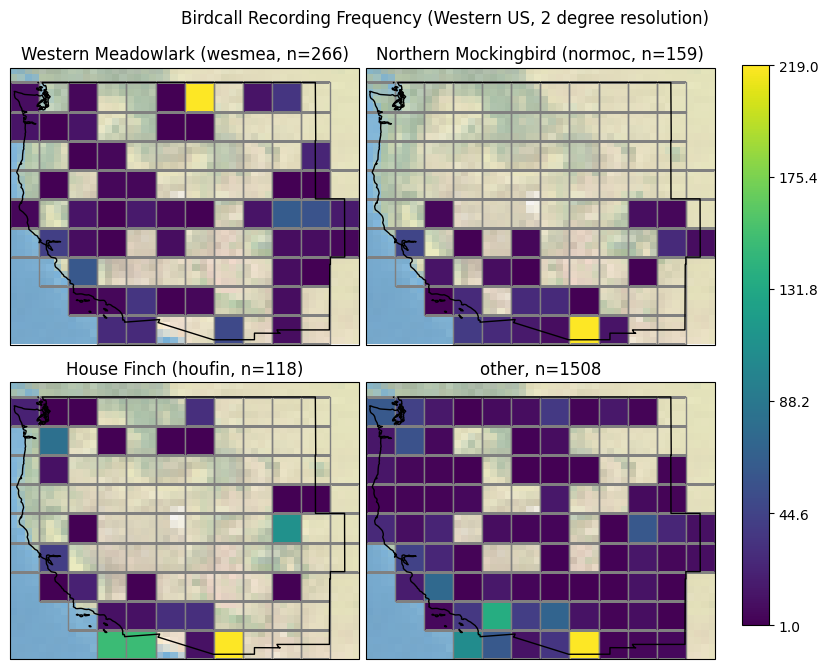
\includegraphics[width=0.8\textwidth]{report/figures/western_us_raw_4.png}
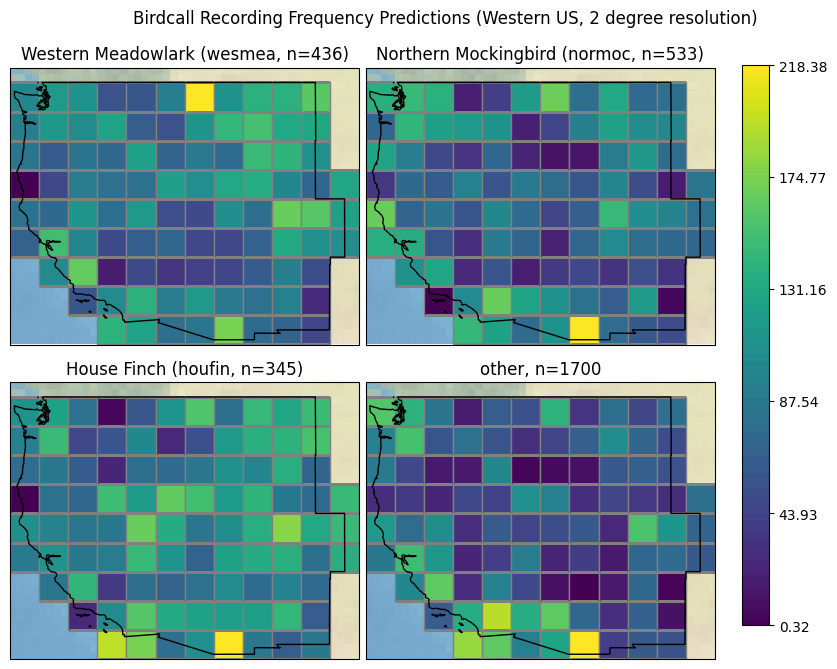
\includegraphics[width=0.8\textwidth]{report/figures/western_us_predict_4.png}
\end{figure}

\begin{figure}[ht!]
\centering
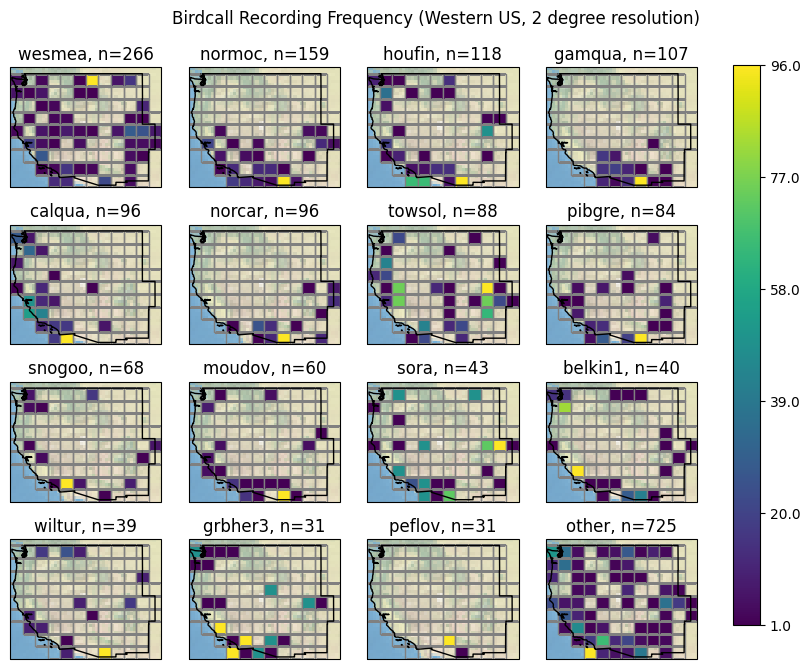
\includegraphics[width=0.8\textwidth]{report/figures/western_us_raw_16.png}
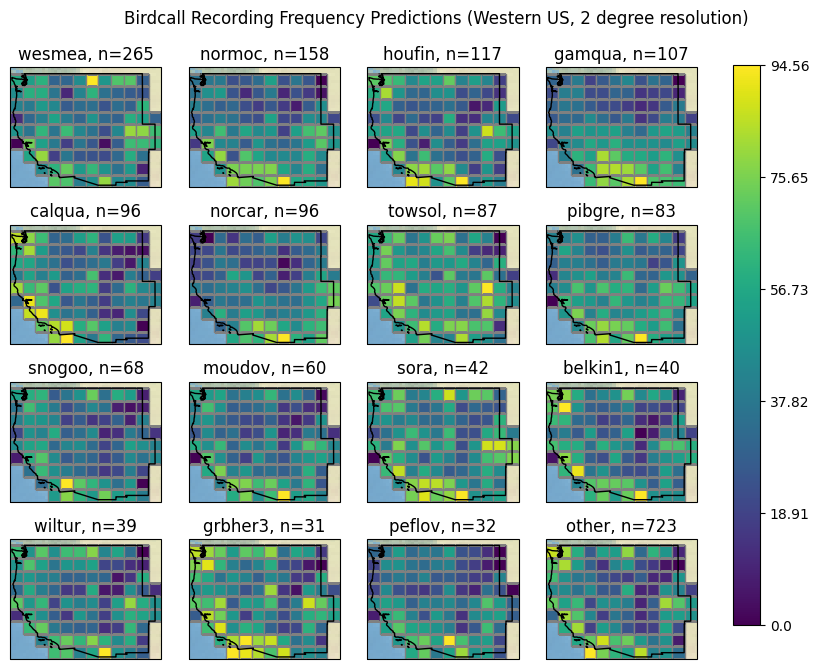
\includegraphics[width=0.8\textwidth]{report/figures/western_us_predict_16.png}
\end{figure}


\section{Discussion}

- Spatial random effects as a form of local smoothing
- Hierarchical modeling as a form of incorporating information across species
- Missing data imputation with distributional assumptions

There are several design choices in the structure of the data and the models that have been left unexplored. One such example is the difference 

\section{Conclusion}

\printbibliography

\end{document}